\section{Introduction}

Viruses are posing increasing threats in the 21st century. 
Researchers and practitioners have proposed a host of tools to prevent?kill? viruses. 
To assist the design of these tools, it is important to understand viruses.

Analyzing the behavior and ** of files that have been compromised in the past
can provide insights into how ***.

%As a free online service, 
VirusTotal~\cite{virustotal} is a popular online service that real-world users use to analyze suspicious files and URLs.
%that analyzes files submitted by real-world users
It applies more than 50 antivirus engines to each submitted file 
to identify various kinds of malwares including viruses, worms, and trojans. 
It then generates a summary report that includes the detection results of all these engines. 
VirusTotal saves and provides an open access of all submitted files and generated reports. 

With the huge amount of real-world files, 
the VirusTotal repository provides a valuable resource to gain insights into 
the behavior of malware.
%Inspired by previous work on mining software repositories~\cite{GuoICSE2010,bigcode, big-lessons,big-translation,code-completion,big-predicting} 
%in the software engineering and programming languages community, 
%we believe that leveraging data on VirusTotal could also enable many ``big security'' applications.   

%The VirusTotal repository provides a valuable resource for conducting data mining. 
First, there is a huge amount of data on VirusTotal.
Figure~\ref{fig:subnum} shows that there were more than 40 million suspicious files 
submitted in November 2015. 
This amount of data makes VirusTotal a rough estimation of malwares in the real world. 
Second, all data on VirusTotal are labeled by state-of-the-art antivirus techniques. 
VirusTotal updates each antivirus engine every five minutes. 
Besides noting whether a given a submitted file has been detected by an antivirus engine, 
VirusTotal also keeps the exact detection tag returned by each engine. 
There are also online active malware researchers 
who can comment and vote on each submitted file 
and thus serve as an important supplement to antivirus engines. 

In industry, antivirus vendors widely use VirusTotal to identify false negatives 
and false positives in their products. 
However, they only utilize VirusTotal reports separately for each single suspicious file, 
failing to consider correlations among different suspicious files. 
In academia, researchers have begun to pay attention to mining the VirusTotal repository. 
For example, ~\citet{neeles} leverage submission\_id information to identify malware writers 
who use VirusTotal as a test platform. 
We believe there are many more research opportunities available through mining VirusTotal. 

In this paper, we conduct an empirical study on the malware dataset on VirusTotal. 
An empirical study is the prerequisite to conduct data mining on VirusTotal. 
We first collect more than 40 million suspicious file submissions from VirusTotal, and then 
we focus our analysis on Windows executable malwares detected by Microsoft
antivirus engine to guarantee accuracy. 
Our analysis includes general characteristics such as submission frequency and the generation rate of malware families, 
temporal characteristics, and family distribution characteristics. 
We hypothesize that malwares do not appear uniformly across time, rather they appear in bursts. 
To validate our hypothesis, we build a cache-based malware prediction technique that aims to predict malwares in which families would appear in the near future. 
Our malware family cache can achieve a 90\% cache hit rate by only using 100 cache entries.
Our technique would allow antivirus vendors to focus their efforts. 
We also observe that distributions of malware families are highly skewed. 
This observation inspires us to apply a frequent item mining algorithm to 
identify hot malware families. 
We view malware submissions as a stream based on their submission timestamps and 
feed this stream into space saving algorithm~\cite{space-saving}. 
Our solution can precisely answer hot malware family queries in nearly-real time, by using a constant number of counters.  


\begin{figure}[t!]
\begin{center}
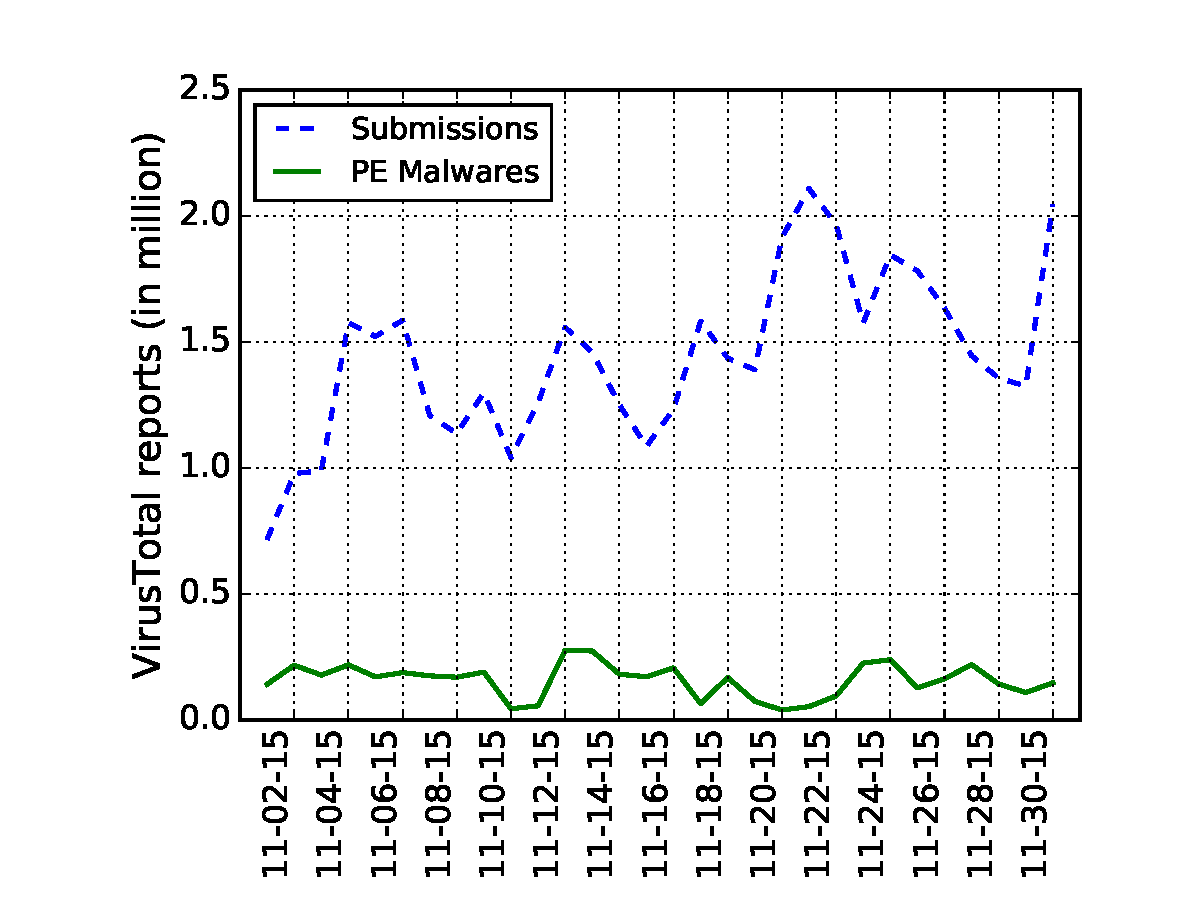
\includegraphics[width=2.5in]{figure/nov}
\caption{The number of suspicious files and the number of malwares submitted to VirusTotal in November 2015. }
\label{fig:subnum}
\end{center}
\end{figure}

To sum up, we make the following contributions in this paper:

\begin{itemize}

\item We collect data submitted to VirusTotal in November 2015 
and analyze their general characteristics. 
We find that most malware samples are only submitted once to VirusTotal (Section~\ref{sec:meth}) 
and that roughly 100-400 new malware families appear each day (Section~\ref{sec:temporal}). 


\item We hypothesize that malwares appear in bursts. 
Our cache-based malware prediction technique confirms our hypothesis, 
and it can achieve greater than 90\% prediction precision (Section~\ref{sec:temporal}). 

\item We observe that family distributions of malwares are highly skewed. 
Leveraging this observation, we build a hot malware family mining technique that can identify hot 
malware families by using a constant number of counters (Section~\ref{sec:dist}).

\item We discuss the future research opportunities available with regard to mining data on VirusTotal (Section~\ref{sec:oppo}). 

\end{itemize}


